\documentclass[12pt,a4paper]{book}
\usepackage[utf8]{inputenc}
\usepackage[portuguese]{babel}
\usepackage[T1]{fontenc}
\usepackage{amsmath}
\usepackage{amsfonts}
\usepackage{amssymb}
\usepackage{makeidx}
\usepackage{graphicx}
\usepackage{booktabs}
\usepackage{color}
\usepackage{hyperref}
\usepackage{float}
\graphicspath{{./Figuras/}}    
\usepackage{multicol}
\definecolor{shadecolor}{rgb}{0.8,0.8,0.8}
\usepackage{amssymb} %Símbolos de Conjuntos numéricos
\usepackage{multicol} %Várias Colunas
\usepackage[left=3cm,right=2cm,top=3cm,bottom=2cm]{geometry}
\author{Leandro Vieira}
\title{Notas de Aula - Física no Ensino Médio}

\begin{document}
\maketitle
\tableofcontents

\chapter{Considerações Iniciais}

%--------------------------------------------------------------------------------------------------------------------------------
%--------------------------------------------------------------------------------------------------------------------------------

%\part{1ª Série do Ensino Médio}

%\part*{I Unidade}

%\part*{II Unidade}

%\part*{III Unidade}

%\part*{IV Unidade}

%--------------------------------------------------------------------------------------------------------------------------------
%--------------------------------------------------------------------------------------------------------------------------------

\part{2ª Série do Ensino Médio}

\part*{I Unidade}

\chapter{Fluídos}
	\section{Densidade}
	
		\newpage \subsection{Problemas e Exercícios}
		\begin{enumerate}
		%QUESTAO 1
		\item Um corpo de massa 1200 kg tem volume igual a $800 m^3$. Calcule a densidade do corpo em $kg/m^3$. Sabendo que $ 1 m^3 = 1.000.000 cm^3$, calcule também a densidade desse corpo em $g/cm^3$:
				
		%QUESTAO 2
		\item Calcule o volume ocupado por um corpo constituído por uma substância cuja densidade é $5,4g/cm^3$, sabendo que sua massa é 250g. Se a massa do corpo for 2 toneladas, qual o volume em $m^3$ ocupado pelo mesmo?
			
		%QUESTAO 3
		\item Calcule o volume em $cm^3$ ocupado por uma porção de ouro cuja massa é 4,0 kg. Calcule também qual a massa de um bloco de ouro com volume $120 cm^3$. (densidade do ouro $19,3 cm^3$ 
		
		%QUESTAO 4
		\item Um tanque cilíndrico é cheio com um óleo cuja densidade é $0,85 g/cm^3$. Sabendo que a altura do tanque é 5 m, e o raio da base do mesmo é 2 m, calcule a massa de óleo contida no tanque. (para calcular o volume do tanque use a fórmula $V=\pi \times r^2 \times h$ onde V é o volume, $r$ o raio, $h$ a altura e $\pi=3,14$)
		
		%QUESTAO 5
		\item Um comerciante recebeu um objeto supostamente feito de ouro puro, com massa 57,9 gramas e volume $2,5 cm^3$. Em dúvida sobre a composição do objeto ele calculou qual a massa de ouro deveria ter o objeto em questão, qual a conclusão do comerciante, mostre os calculos que permitiram essa conclusão. 
		
		%QUESTAO 6
		\item Uma solução cuja densidade é de 1150 g/L foi preparada, dissolvendo-se 160 g de NaOH em $760 cm^3$ de água. Determine respectivamente a massa da solução obtida e seu volume. (Dados: densidade da água = $1,0 cm^3$, 1 litro = $1.000 cm^3$)
		
		%QUESTAO 7
		\item Qual a densidade em $g/cm^3$ de uma solução de volume igual a 5 L e massa de 4,0 kg:
		
		%QUESTAO 8
		\item Uma solução foi preparada misturando-se 30 gramas de um sal em 300 g de água. Considerando-se que o volume da solução é igual a 300 mL, a densidade dessa solução em g/mL será de:
		
		%QUESTAO 9
		\item A densidade do diamante é $3,5 g/cm^3$. A unidade prática internacional para a pesagem de diamantes é o quilate, que corresponde a 200 mg. Qual o volume de um diamante de 1,5 quilate
		
		%QUESTAO 10
		\item Um líquido, com volume de 10,7 mL, tem a massa de 9,42 g. O líquido pode ser octano, etanol ou benzeno, cujas densidades são, respectivamente (em $g/cm^3$), 0,702, 0,789 e 0,879. Qual é o líquido? Justifique a resposta.
		
		%QUESTAO 11
		\item Um sólido flutuará em um líquido que for mais denso do que ele. O volume de uma amostra de calcita pesando 35,6 g é 12,9 $g/cm^3$. Em qual dos seguintes líquidos haverá flutuação da calcita: Tetracloreto de carbono (densidade = 1,60 $g/cm^3$), brometo de metileno (densidade = 2,50 $g/cm^3$), tetrabromoetano (densidade = 2,96 $g/cm^3$) ou iodeto de metileno (densidade = $g/cm^3$)? Justifique a resposta:
		
		%QUESTAO 12
		\item Dois líquidos, A e B, quimicamente inertes, e não-miscíveis entre si, de densidades dA=2,80$g/cm^3$ e dB=1,60$g/cm^3$, respectivamente, são colocados em um mesmo recipiente. Sabendo que o volume do líquido A é o dobro do de B, a densidade da mistura, em $g/cm^3$, vale:
		
		%QUESTAO 13
		\item Um bloco de ferro ($d= 7,6 g/cm^3$) tem as seguintes dimensões: 20cm x 30cm x 15cm. Determine a massa, em kg, do bloco:
		\end{enumerate}
	
	
	\newpage \section{Princípio de Arquimedes}
		
		\newpage \subsection{Problemas e Exercícios}
		
		
		\begin{enumerate}
		
		%QUESTAO 1
		\item Um objeto com massa de 10 $kg$ e volume de 0,002 $m^3$ é colocado totalmente dentro da água:
		
		\par a) Qual é a intensidade da força de empuxo que a água exerce no objeto:		
		\par b) Qual o valor do peso aparente do objeto:
		
		%QUESTAO 2
		\item Qual a intensidade do empuxo sobre um bloco de aço com 0,4 $m^3$ de volume no fundo de um tanque de gasolina: Qual o valor do peso aparente desse bloco:
		
		%QUESTÃO 3
		\item Calcule o peso aparente de uma pedra, cuja massa é 150 $kg$, quando colocada no fundo de uma piscina com água, dado o volume da pedra V = 0,064 $m^3$. 
				
		%QUESTAO 4
		\item O empuxo em uma barra de alumínio submerso é de 850 N. Calcule:
		\par a) O volume da barra e sua massa, sabendo que a densidade do alumínio é $2,7 \times 10^3$ $kg/m^3$:
		\par b) Qual o peso aparente desse bloco quando ele está dentro de um tanque de água? E dentro de um tanque de gasolina?
			
		%QUESTAO 5
		\item A densidade do ouro é $1,93 \times 10^3$ $kg/m^3$, com o intuito de calcular a massa de um objeto irregular, um ourives percebeu que o peso aparente do mesmo era 0,5 N. Qual a massa do objeto:
		
		%QUESTAO 6
		\item Um tanque é cheio com um óleo cuja densidade é 850 $kg/m^3$. Dentro do tanque há um bloco de concreto cuja massa é 50 kg e um bloco de aço cujo volume é 0,08 $m^3$:
		\par a) Qual o empuxo sobre os objetos?
		\par b) Calcule o peso aparente dos objetos?
		
		%QUESTAO 7
		\item O peso aparente de um objeto cuja massa é 50 $kg$ em um tanque cheio com um determinado fluído é 450 N. Calcule Qual a densidade do fluído, uma vez que o volume do objeto é 0,045 $m^3$:
		
		%QUESTÃO 8
		\item Qual o peso aparente de uma pessoa, com massa 75 $kg$, quando ela está na água. (a massa específica do ser humano é 1.010 $kg/m^3$)
		
		%QUESTAO 9
		\item O peso aparente de um objeto na água é 25 N. Sabendo que esse objeto é feito de um substância cuja massa específica é 1.250 $kg/m^3$, calcule o a massa e o volume do objeto: 
		
		%QUESTAO 10 
		\item Qual o peso aparente de um bloco de concreto com 1,0 $m^3$ que está submerso. (densidade do concreto 2.500 $kg/m^3$:
				
\end{enumerate}		
	
%--------------------------------------------------------------------------------------------------------------------------------

\part*{II Unidade}
\chapter{Estudo dos Gases}

	\section{A Equação de Clapeyron}

		\newpage \subsection{Problemas e Exercícios}
		
\begin{enumerate}
\item A massa molar do gás O2 (oxigênio) é 32 g. Calcule 
\newline a)	A quantidade de moles em de 2kg de oxigênio:
\newline b)	A Massa equivalente a uma quantidade de 120 moles de O2: 
\item  Qual a pressão de 2kg de oxigênio, à temperatura de 200 K que ocupa um espaço de 50 l. 
\item  Calcule a temperatura de 320 g de oxigênio que ao ocupar um volume de 20 l está sob uma pressão de 4,5 atm.
\item  A massa de 500g de certo gás de molécula grama 25 g (M = 25 g), ocupa o volume de 16 l. 
\newline a)	Calcule a pressão desse gás à temperatura de 120 K e 400 K:
\newline b)	A temperatura do gás à pressão de 5 atm e de 8 atm. 
\item  Calcule o número de moles de um gás que à temperatura de 420 K ocupa o volume de 20 l com pressão de 10 atm.
\item  Calcule a temperatura de 450 g de oxigênio que ao ocupar um volume de 40 l está sob uma pressão de 2,5 atm.
\item  A massa de 200g de certo gás de molécula grama 16 g (M = 16 g), ocupa o volume de 6 l. 
\newline a)	Calcule a pressão desse gás à temperatura de 10 K e 300 K:
\newline b)	A temperatura do gás à pressão de 6 atm e de 10 atm. 
\item  Calcule o número de moles de um gás que à temperatura de 200 K ocupa o volume de 25 l com pressão de 20 atm.
\item  Um balão com 2,00 litros de capacidade, ao se elevar do solo contém 80 g de hélio à temperatura de 17 C. Nessas condições, a pressão exercida pelo gás no interior do balão é: (Massa molar do gás hélio é 4 g).
\item  Calcule a pressão em um botijão à temperatura de 25 C de gás que contém 13 kg de butano, cujo volume é 20 l. Massa molar do butano 58,12 g.
\item  Calcule o número de moles em uma massa de certo gás que às condições normais de temperatura e pressão ocupa o volume de 10 l.
\item  Qual o volume que ocupa 1,5 kg de butano com uma pressão de 5 atm, estando à temperatura de 20 C
\end{enumerate}

	\newpage \section{As Transformações Gasosas}

		\newpage \subsection{Problemas e Exercícios}
		
\begin{enumerate}
\item Em um recipiente fechado, certa massa de gás ideal ocupa um volume de 12 litros a 293k. Se este gás for aquecido até 302k, sob pressão constante, seu volume será:
\item Um recipiente indeformável, hermeticamente fechado, contém 10 litros de um gás perfeito a 30 C, suportando a pressão de 2 atmosferas. A temperatura do gás é aumentada até atingir 60 C.
\newline a)	Calcule a pressão final do gás.
\newline b)	Qual a temperatura do gás caso a pressão passe para 5 atm:
\item A 27 C, um gás ideal ocupa 1,5 litro. Que volume ocupará a – 73 C, sendo a transformação isobárica?
\item Quinze litros de uma determinada massa gasosa encontram-se a uma pressão de 8,0 atm e à temperatura de 30 C. Ao sofrer uma expansão isotérmica, seu volume passa a 20 litros. Qual será a nova pressão do gás?
\item Um pneu foi regulado para manter uma 1,5 atm, a uma temperatura de 14 C. Durante o movimento do automóvel, no entanto, a temperatura do pneu elevou-se a 55 C. Determine a pressão interna correspondente.
\item Um carro-tanque transportou gás cloro para uma estação de tratamento de água. Sabe-se que o volume do tanque que continha gás cloro era de 30 m3, que a temperatura era mantida a 20oC para a pressão ser de 2 atm e que, na estação de tratamento de água, esse cloro foi transferido para um reservatório de 50 m3 mantido a 293 K. Qual a transformação gasosa sofrida pelo gás? Qual a pressão final do gás?
\item Antes de realizar uma viagem de carro, em um dia cuja temperatura era de 30oC, um senhor calibrou os pneus utilizando 3 atm de pressão. Quando chegou ao destino, depois de 5 horas de viagem, mediu novamente a pressão dos pneus e constatou 3,4 atm de pressão. Sabendo que a variação de volume dos pneus é desprezível, calcule a temperatura em que se encontravam os pneus ao fim da viagem:
\item Uma empresa pretende utilizar balões para realizar uma operação de publicidade em uma praia. Os balões foram preenchidos com uma pressão de 760 mmHg, a uma temperatura de 32 oC. Ao chegar à praia, a temperatura estava em 42oC, mas a pressão ainda era de 760 mmHg. Quantas vezes o volume dos balões foi alterado ao chegar à praia?
\item Pela manhã, um motorista calibra os pneus de seu carro sob uma pressão de 28,0 lb/pol2 quando a temperatura era de 7 C. À tarde, após rodar bastante, a temperatura dos pneus passou a ser 37 C. Considerando que o volume dos pneus se mantém constante e que o comportamento do ar seja de um gás ideal, a pressão nos pneus aquecidos, em lb/pol2, passou a ser. 
\item No início do curso de compressão, o cilindro de um motor diesel contém 800 cm de ar, à pressão atmosférica (1 atm) e à temperatura de 27 C. No fim desse curso, o volume de ar foi reduzido para 50 cm e a pressão manométrica aumentada para 40 atm. A variação de temperatura da massa de ar no cilindro foi de: 

\end{enumerate}


%------------------------------------------------------------------------------------------------------------------------------
\chapter{Calorimetria}

	\newpage \section{Problemas e Exercícios}
	
\begin{enumerate}
\item Qual a capacidade térmica de um corpo que ao receber 4 kcal, teve um aumento de 25 C em sua temperatura:
\item  Um corpo de massa 500 g, ao receber 8 kcal teve um aumento de 50C em sua temperatura, calcule:
\newline a)	Capacidade térmica desse corpo:
\newline b) O calor específico da matéria que o compõe:
\newline c) A quantidade de calor necessário para elevar em 120 C a temperatura de 1,0 kg do material desse corpo:
\item Uma barra de ferro com 50 kg (c = 0,113 cal/g ), recebeu 150 kcal de energia térmica. Calcule a variação na temperatura dessa barra:
\item Calcule a massa de um bloco de vidro (c = 0,020 cal/g C) que sofreu um aumento de 36 C em sua temperatura ao receber 12 kcal:
\item  Uma barra de ferro de comprimento 20 m (2.000 cm), ao ser aquecida teve uma dilatação linear de 2,5 cm.
\newline a)	Calcule a variação na temperatura da barra, sabendo que para o ferro C-1:
\newline b)	A massa da barra é 30 kg, calcule a quantidade de calor que essa barra recebeu.
\item  Um bloco de ferro com volume 20.000 cm de volume, tem massa 157 kg. O bloco em questão recebeu 5.500 kcal de energia térmica.
\newline a)	Calcule a variação na temperatura desse bloco:
\newline b)	Qual a dilatação volumétrica do bloco:
\item  Calcule a dilatação em um fio de ferro de comprimento 100 m que recebeu 4 kcal. A massa do fio é 2 kg. 
\end{enumerate}

%--------------------------------------------------------------------------------------------------------------------------------
\chapter{Princípios de Termodinâmica}

A Primeira coisa a ser dita sobre termodiâmica é que esta palavra deriva de dinâmica, ramo da física que lida com a matéria em movimento.

	\section{Dinâmica}
A dinâmica é o estudo da causa do movimento. Parte da física fundamentada no trabalho de Isaac Newton (1642-1727), tem como um de seus produtos finais as três leis a seguir, também conhecidas como Leis de Newton:

		\subsection{Primeira Lei Newton (Lei da Inércia de Galileu)}
Essa lei fala da inércia, atributo essencial, da matéria. A inércia é a propriendade que a matéria tem de ser incapaz de mudar sua posição em relação a um referencial sem intervenção de outros objetos. Essa lei afirma que todo corpo em repouso tende a ficar em repouso, a não ser que uma força incida sobre o mesmo. O mesmo valendo para corpos em movimento, que tendem a continuar em movimento com velocidade constate e em linha reta a não ser que uma força aja sobre o mesmo.

A Lei da Inércia pode ser exemplificada com os saélites que orbitam a terra. Após lanaçados os mesmo mantê-se em constante movimento, tendo como lastro a força da gravidade que os mantêm em movimento em torno da terra. Outro exemplo vem ao empurar objetos em superfícies planas e lisas, em uma escala real, é impossível não considerar o atrito, seja do ojeto com a superfície, ou mesmo do objeto com o ar, no entanto para situações em pequena escala, se nota que nesse tipo de lançamento, o objeto, para apenas ao encontrar outro objeto, seja uma parede, seja uma pessoa, etc.. 

A interação entre objetos se dá atravez de uma força. Apesar da dificuldade em definir o conceito de força , nota-se que a força está intimamente ligado com mudanças na matéria, na situação em questão, as mudanças na matéria são ralativas à mudança de posição em relação um referencial dado. Em outras palavras, a força é capacidade de por em movimento ou em mudar o movimento de um corpo dado.

		\subsection{Segunda Lei de Newton}

Essa lei exprime a proporcionalidade entre força e aceleração. Que resulta na seguinte equação: 

$$\vec{F}=m.\vec{a}$$

Nessa equação a unidade de força a o newton (N), as unidade de massa e aceleração estão no S.I., e são respectivamente kg e $m/s^{2}$.

obs.: A notação de vetor $\vec{F}$ e $\vec{a}$, não deve causar muita complicação, pois para o estudo em questão consideraremos situações em que a força e a aceleração tem o mesmo sentido. 

A Segunda Lei é base para uma série de aplicações da dinâmica à situações cotidianas. Uma dessas envolve a definição de trabalho realizado por uma força. Definimos o trabalho como o produto do módulo da força pelo deslocamento, quando a força e aceleração tem a mesma direção:

$$ W = F \cdot d$$

Onde $d$ é o deslocamento do corpo causado pela força $F$

Da equação $\vec{F}=m.\vec{a}$, e do da definição de aceleração como $ a = \frac{\Delta v}{\Delta t}$, vem a equação:

$$ F = \frac{m \cdot \Delta v}{\Delta t}$$

Para um instante dado, onde a velocidade é $v$, temos $p = m \cdot v$, que é chamado momentum do corpo de massa m, cuja velocidade é v.

Quando a força e a aceleração estão no S.I., a unidade do trabalho é o joule (J). Assim força também pode ser definida como a capacidade de realizar um trabalho, sendo necessário tanto mais força para realizar trabalhos maiores. 

{Nesse ponto inserir alguns exercícios sobre a segunda lei}

				\subparagraph{Exemplo 1} Sobre um Bloco A de massa 10 kg há aplicação de uma força F, conforme indicado na figura a seguir

%\begin{figure}[h]
%\center
%\includegraphics[width=8cm]{Figuras/Q1.png}
%\label{omeubrowser}
%\end{figure}

Sabendo que a aceleração do bloco é 2 $m/s^2$, calcule:

a) A o módulo da força aplicada sobre o bloco:

b) Uma vez que sob essa força, o bloco se deslocou 20 m, calcule o trabalho realizado pela mesma:

				\subparagraph{Exemplo 2} Uma força $\vec{F}$ é aplicada sobre um bloco B, como indicado abaixo. Sabendo que o bloco se move 16m. Calcule o trabalho realizado pela força.

%\begin{figure}[h]
%\center
%\includegraphics[width=8cm]{Figuras/Q1.png}
%\label{omeubrowser}
%\end{figure}

			\subsubsection{Aplicações da Segunda Lei - Força não Paralela ao Deslocamento}

			\subsubsection{Aplicações da Segunda Lei - Plano Inclinado}

			\subsubsection{Aplicações da Segunda Lei - Várias Forças Sobre um Mesmo objeto}

			\subsection{Terceira Lei de Newton - Lei da Ação e da Reação}

	\section{Termodinâmica I} 

No Século XVIII surgem as primerias máquinas a vapor. Nessas máquinas o vapor entra em um cilindro empurrando um pistão transformando o calor em trabalho.

%\begin{figure}[h]
%\center
%\includegraphics[width=8cm]{termo1fig1.png}
%\label{omeubrowser}
%\end{figure} 

		\subsection{Trabalho em Uma Transformação Gasosa}

Seja um cilindro e um pistão como os da figura a seguir. O gás dentro do cilindro exerce uma força $\vec{F_G}$ sobre o pistão de área $A$ conforme a figura, e essa força é medida pela pressão $p$ sobre o pistão , ao aquecer o gás, o pistão se desloca $d$ unidades para cima, havendo uma variação $\Delta V$ no volume incial do gás. Para, a força temos:

$$W=F_G \cdot d$$

Mas $p=\frac{F}{A}$, e daí vem  $F=p \cdot A$, e por outro lado temos também $\Delta V = A \cdot d$. Assim:

$$W=F_G \cdot d = p \cdot A \cdot d = p \cdot \Delta V$$

Obs.: nessa situação trabalharemos com a pressão e o volume no S.I., ou seja, a pressão em Pa (pascal), e o volume em $m^3$. Temos $ 1 atm \cong 10^5 Pa$ e $ 1 m^3 = 1000 litros$.

			\subparagraph{Exemplo 1}: Uma porcão de um gás ideal sob pressão de 0,2 atm sofre uma transformação isobárica. Sabendo que o aumento no volume do gás foi de 2,4 litros, calcule o trabalho realizado pelo gás nessa transformação:
			
			\subparagraph{Exemplo 2}: Calcule a variação no volume de uma porção de um gás ideal que ao sofrer uma transformação isobárica realizou um trabalho de 2500J(dados pressão do gás 1600 Pa):

	\newpage \section{Problemas e Exercícios - Dinâmica e Termodiâmica I} 

\begin{enumerate}
\item Uma força F incide sobre um objeto de massa 5,0 kg, calcule o módulo de F, uma vez que a aceleração do objeto é de 2,4 $m/s^2$:
\item Qual a aceleração de um objeto de massa 800 kg sobre o qual uma força de intensidade 200N é exercida:
\item Uma força F aplicada sobre um bloco de massa 2,0 kg produz uma aceleração de 3,4 $m/s^2$. Calcule o trabalho realizado, uma \item  que o bloco foi deslocado por essa força por 5 m:
\item  Uma força executa um trabalho de 1600 J, ao deslocar um objeto de massa 2,5 kg, 4 m. Calcule a aceleração do objeto durante o percurso.
\item  Calcule o trabalho realizado sobre o bloco A e B, de massa $m_A = 4,0$ kg e $m_B = 4,5$ kg, indicados nas figuras a seguir, ambas foram deslocadas 10 m:

	\begin{figure}[h]
	\center
	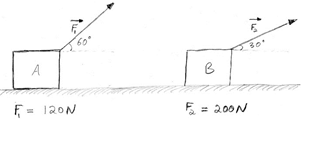
\includegraphics[width=8cm]{dinamica1ex1.png}
	\label{omeubrowser}
	\end{figure}

\item  Calcule o trabalho realizado por um gás que sofreu uma variação de 10 litros em seu volume inicial, ao passar por uma transformação isobárica. A pressão é 2500 Pa.
\item  Um gás realizou um trabalho de 3200 J ao se expandir 10 litros. Calcule a pressão do gás em atm:
\item  Qual foi a variação no volume de um gás que ao expandiu 50 litros, e manteve sua pressão constante em 0,05 atm, quanto teve sua temperatura variada.  
\item  Ao se expandir 25 litros um gás realizou um trabalho de 4000 J. Sabendo que a pressão do gás se manteve constate, calcule-a:
\item  Se um gás que passar por uma transformação isobárica expandir 2,4 litros, qual será o trabalho realizado por ele uma vez que sua pressão é 1 atm.
\item  Calcule a variação no volume de um gás que manteve a temperatura constante em 0,4 atm, enquanto realizava um trabalho de 5000 J numa transformação gasosa:

\end{enumerate}

	\newpage \section{Termodinâmica II}
	\newpage \section{Problemas e Exercícios - Termodiâmica II}
	
\begin{enumerate}
\item Calcule a pressão de um gás que ocupa um volume de 50 litros e tem energia interna de 1.500 J:
\item A pressão de um gás é de 0,25 atm e sua energia interna é 2400 J. Qual o volume ocupado por ele:
\item Qual a energia interna de uma gás que ocupa o volume de 25 litros sob pressão de 2,5 atm:
\item Um gás expande, realizando um trabalho de 1200 J, sabendo que o gás recebeu 2500 J de energia térmica, calcule a variação na energia interna do gás:
\item Um gás expandiu 8 litros ao passar por uma transformação isobárica. Sabendo que a pressão do gás é 2 atm, calcule:
\newline a)	O trabalho realizado pelo gás:
\newline b)	Sabendo que o volume inicial do gás é 50 litros, calcule a variação na energia interna do gás:
\newline c)	Qual a quantidade de calor que o gás recebeu durante esse processo:
\item Um gás recebeu 2.000 J de energia térmica, ao receber essa energia o gás realizou um trabalho de 800 J. Calcule a energia interna do gás após receber energia térmica, uma vez que a pressão e o volume iniciais do gás são respectivamente 400 Pa e 0,025 $m^3$: 
\item Sabendo que a pressão de um gás é 160 Pa, calcule a variação no volume do gás que ao receber 4.000 J de calor, teve um aumento de 1800 J em sua energia Interna:
\item Ao passar por uma transformação Isobárica, certa massa de gás à pressão de 250 Pa, teve um aumento no volume de 2 litros, calcule a quantidade de calor recebido pelo gás, uma vez que o mesmo teve um aumento de 800 J em sua energia interna:
\item Calcule a pressão de um gás que ao receber durante uma transformação isobárica 3000 J de energia térmica, sofre um aumento de 10 litros em seu volume e de 1400 J em sua energia Interna: 
\end{enumerate}	 
%--------------------------------------------------------------------------------------------------------------------------------
%III Unidade - 2 ano

\part*{III Unidade}

\chapter{Ondulatória}
	\section{Movimento Harmônico Simples}
	
	\section{Ondas}
		\subsection{Ondas Eletromagnéticas}
	
	\section{Acústica}
	
\part*{IV Unidade}
%--------------------------------------------------------------------------------------------------------------------------------
%IV Unidade - 2 ano
\chapter{Óptica Geométrica}
	\section{Conceitos Iniciais}
	\section{Reflexão da Luz}
		\subsection{Espelhos Planos}
		\subsection{Espelhos Esféricos}
	\section{Refração da Luz}


\part{3ª Série do Ensino Médio}
%--------------------------------------------------------------------------------------------------------------------------------

%Capítulos do Terceiro Ano

%--------------------------------------------------------------------------------------------------------------------------------
\part*{I Unidade}
%I Unidade - 3 ano
\chapter{Eletrostática}

	\section{Lei de Coulomb}
		\newpage \subsection{Problemas e Exercícios}
	
	\begin{enumerate}
		
	%QUESTAO 1
	\item Dois corpos $A$, e $B$ estão distanciados $2,5$ $m$ no vácuo. Sabendo que a carga de A é $-2,5 \cdot 10^{-4}$ $C	$,e que a carga de B é $4,5 \cdot 10^{-4}$ $C$; diga se a força entre os dois corpos é de atração ou repulsão e calcule seu 	módulo:
		
	%QUESTAO 2
	\item Calcule o módulo da força de repulsão entre dois corpos $A$, e $B$, de cargas iguais a $1,5 \cdot 10^{-5}$ $C$, 	sabendo que ambos se encontram a $0,25$ $m$ um do outro.
		
	%QUESTAO 3
	\item A distância entre o próton e o elétron no átomo de hidrogênio é da ordem $5,3 \cdot 10^{-11}$ $m$. Calcule a força de repulsão entre o próton e o elétron no núcleo de hidrogênio, uma vez que a carga do elétro é $-1,6 \cdot 10^{-19}$ $C$ e a carga do próton é $1,6 \cdot 10^{-19}$ $C$: 
	
	%QUESTAO 4
	\item Um corpo eletricamente neutro A sofreu um processo de eletrização, ganhando $4,5 \cdot 10^{23}$, e outro corpo B, também eletricamente neutro perdeu em outro processo de eletrização perdeu $5,4 \cdot 10^{23}$ elétrons. Após a eletretrizão dos corpos A e B, os mesmos foram colocados a uma distância de $0,4$ $m$ no vácuo.
	\par a) Qual a carga do corpo e do corpo A e do B? A força entre eles é de atração ou repulsão?
	\par b) Qual o módulo da força entre eles?
	
	%QUESTAO 5
	\item Duas cargas puntiformes $Q_{1} = 1,5 \cdot 10^{-4}$ $C$ e $Q_{2} = 4 \cdot 10^{-4}$ $C$ estão distanciadas no vácuo, e a força entre elas é de $1,6$ $N$, calcule a distância entre elas:
	
	%QUESTAO 6
	\item Calcule a distância entre duas cargas iguais a $Q = 5,2 \cdot 10^{-4}$, sabendo que a força de repulsão entre elas é de $2,5$ $N$:

	%QUESTAO 7
	\item Duas cargas iguais estão distanciadas $3$ $m$ no vácuo. Sabendo que a força de repulsão entra elas é $2$ $N$ calcule o valor das duas cargas:
	
	%QUESTAO 8 
	\item Calcule a distância que deve haver entre duas cargas iguais a $Q = 5,2 \cdot 10^{-4}$ no vácuo para que a força de repulsão entre elas seja de $5$ $N$: 
	
	%QUESTAO 9
	\item Dois corpos $A$ e $B$ eletrizados positivamente estão distanciados $0,25$ $m$ no vácuo. Sabendo que que a força de repulsão entre eles é de $0,2$ $N$. Calcule o valor da carga de cada um dos corpos, uma vez que a carga de $A$ é $2Q$ e a carga de $B$ é $Q$
	
	%QUESTAO 10
	\item Duas gargas puntiformes $Q_{1}=2,5$ $\mu C$, $Q_{2}=2,1$ $\mu C$ estão distanciadas $0,2$ $m$ no vácuo. Calcule o valor da força de repulsão entre essas duas cargas. 
	
	%QUESTAO 11
	\item Qual a quantidade de elétrons que um corpo deve perder para que sua carga seja de $2,5$ $\mu C$:
	
	%QUESTAO 12
	\item Uma carga puntiforme $Q_{1} = 4,2 \cdot 10^{-5}C$ está distanciada $0,5$ $m$ no vácuo de um segunda carga $Q_{2}$. Sabendo que a força de atração entre essas duas cargas é de $2,4$ $N$, calcule o valor de $Q_{2}$:
	
	%QUESTAO 13
	\item Calcule a quantidade de elétrons que um corpo deve ganhar para que sua carga seja de $-9,8$ $\mu C$:
	
	%QUESTAO 14
	\item Qual deve ser o valor de um carga $Q_{1}$, para que quando distanciada $0,25$ $m$ de uma segunda carga $Q_{2} = 1,6 \cdot 10^{-4}$, no vácuo haja entre elas uma força de repulsão de $2,4$ $N$:

	\end{enumerate}
	
	\newpage \section{Campo Elétrico}
		\section{Potencial Eletrostático}
		
		\newpage \section{Problemas e Exercícios}	
		
	\begin{enumerate}
		
	%QUESTAO 1
	
	\item Uma carga de intensidade $2,5 \cdot 10^{-5}$ $C$ é colocada em um ponto do campo elétrico produzido por uma carga puntiforme $Q$, cuja intensidade é $4,2 \cdot 10^{-4}$ $N/C$. Calcule o módulo da força de repulsão entre as duas cargas:
		
	%QUESTAO 2
	\item Calcule o módulo da força de repulsão gerado por um campo elétrico de intensidade $5,0 \cdot 10^{-5}$ $N/C$, sobre uma carga $q$ de intensidade $1,4 \cdot 10^{-5}$ $C$:
		
	%QUESTAO 3
	\item Uma carga $q$, de intensidade $2,5 \cdot 10^{-5}$ $C$ é colocado em ponto de um campo elétrico, sabendo que a força constatada foi da ordem de $4,4 \cdot 10^{-10}$ $N$, calcule a intensidade do campo elétrico:
	
	%QUESTAO 4
	\item Qual a intensidade de um campo elétrico, que gera uma força de atração de módulo  $5,6 \cdot 10^{-12}$ $N$ sobre um carga puntiforme  $q = 1,6 \cdot 10^{-7}$ $C$
	
	%QUESTAO 5
	\item Qual deve ser a intensidade de uma carga $q$ para que ao ser colocada no ponto de um campo elétrico de intensidade $3,4 \cdot 10^{-8}$ $N/C$ gere uma força de intensidade $F = 1,7 \cdot 10^{-12}$ $C$
	
	%QUESTAO 6
	\item Calcule a intensidade de uma carga puntiforme $q$ para que um campo elétrico de intensidade $4,5 \cdot 10^{-9}$ $N/C$ gere sobre $q$ uma força de repulsão da ordem de $3,0 \cdot 10^{-15}$ $N$ 
	
	%QUESTAO 7
	\item Qual a intensidade do campo elétrico gerado por uma carga puntiforme $Q = 6,5 \cdot 10^{-7}$ $C$, na região do espaço situado a 2 m da mesma:
	
	%QUESTAO 8 
	\item Uma carga $Q = 9,3 \cdot 10^{-6}$ $C$ gera um campo elétrico com qual módulo na região distante da mesma 2,5 m:
	
	%QUESTAO 9 
	\item Qual deve ser a intensidade de uma carga $Q$ para que o campo gerado pela mesma num ponto distante 1,6 m tenha intensidade $2,4 \cdot 10^{-9}$ $N/C$:
	
	%QUESTAO 10
	\item Calcule a intensidade de uma carga puntiforme $Q$ que gera um campo de intensidade $4,2 \cdot 10^{-10}$ $N/C$, num ponto que situa a 1,2 m da mesma:
	
	%QUESTAO 11
	\item Em qual distância de uma carga pontual $Q = 1,4 \cdot 10^{-4}$ $C$, há um campo elétrico de intensidade  $4 \cdot 10^{-10}$ $N/C$:
	
	%QUESTAO 12
	\item Em uma região do plano, uma carga pontual $Q = 2,5 \cdot 10^{-12}$ $C$, gera um campo elétrico de intensidade  $1,6 \cdot 10^{-2}$ $N/C$. Calcule a distância que essa região se encontra da carga $Q$:
	
	%QUESTAO 13
	\item Qual a distância que uma região no plano se encontra de uma carga $Q = 1,5 \cdot 10^{-4}$ $C$, sabendo que nessa região há um campo elétrico gerado por $Q$ de intensidade $2,4 \cdot 10^{-3}$ $N/C$:
	
	%QUESTAO 14
	\item Calcule a distância que uma região se encontra de uma carga puntiforme $Q$, sabendo que o valor do campo elétrico gerado por $Q$ tem intensidade $4,5 \cdot 10^{-2}$ $N/C$. Dado $Q = 3,5 \cdot 10^{-3}$ $C$ 
			
	\end{enumerate}

%--------------------------------------------------------------------------------------------------------------------------------
%II Unidade - 3 ano

\part*{II Unidade}
\chapter{Eletrodinâmica}

	\section{Intensidade de Corrente Elétrica}
		
		\subsection{Energia e Potência}




		\subsection{Diferença de Potencial}

	\section{Resistores}
	
		\subsection{Lei de Joule}

A Lei de Joule quantifica a tranformação de energia elétrica em enregia térmica realizada por um resistor. Essa transformação é dada pela seguinte fórmula:

				$$\mathrm{E} = R \cdot i^2 \cdot \Delta T$$	

Onde $\mathrm{E}$ é a energia convertida em joule (J), pelo resistor de resistência $R$ (em $\Omega$), o qual é utrapassado por uma corrente elétrica de intensidade $i$ (em ampers). A quantidade de energia convertida depende do tempo $\Delta T$ em que o resisitor é ultrapassado pela corrente. Note que todas as medidas estão no S.I.. 

Essa fórmula é muito usada em combinação com equação fundamental da calorimetria $\mathrm{Q} = \mathrm{c} \cdot m \cdot \Delta t$ que quantifica a variação na temperatura de um corpo ($\Delta t$) de massa $m$ em função da quantidade de calor $Q$ recebido pelo mesmo, c é uma constante específica do material que constitui o corpo, é chamada de calor específico. Nessa fórmula, o calor geralmente é medido em cal, quando necessário a conversão, pode-se usar:

				$$ 1 \mathrm{cal} = 4,2 J$$

			\paragraph{Exemplo} Um resistor de $2,5 \Omega$ é colocado dentro de um recipiente contendo 10 kg de água. Sabendo que o resistor está submetido a uma d.d.p. de 100 V, calcule a variação na temperatura da água se o resistor ficar 2 min dentro do recipiente:
			
		\subsection{Potência}

A potência dissipada por um resistor é dado pela fórmula a seguir:

$$ \mathrm{P} = \frac{\mathrm{U}^2}{\mathrm{R}}$$

Na fórmula anterior P é dado em walt (W), U é a d.d.p. à qual o resistor de resitência R está submetido. A partir dessa fórmula obtemos uma outra maneira de quantificar a energia dissipada por um resistor:

$$ \mathrm{E} = \mathrm{P} \cdot \Delta T$$

Note que usando o tempo em horas obtemos a energia em Wh, essa unidade de medida é bastante usada na eletricidade.

			\paragraph{Exemplo 1} Em um chuveiro elétrico está escrito 2.200 W - 220 V. Sob essas condições calcule:
			\paragraph{} a) Qual a intensidade da corrente que o atravessa: 
			\paragraph{} b) Qual a resitência do chuveiro:
			\paragraph{} c) Qual o consumo desse chuveiro após 12 min de uso:			
			
			\paragraph{Exemplo 2} Em um chuveiro está escrito 3300 W - 220 V. Calcule a energia consumida em kWh por esse chuveiro após 12 min de uso.
			
			\paragraph{Exemplo 3} Um resitor de 5$\Omega$ permite a passagem de uma corrente de 50 A sob uma determinada d.d.p. Calcule a energia consumida por esse resitor após 30 min de uso:
			
	\section{Associação de Resistores}

%--------------------------------------------------------------------------------------------------------------------------------
\part{Anexos}
\chapter{Conteúdo Programático Física do Ensino Médio - PE}
	\section{Introdução}
	\section{Conteúdo Programático}
		\subsection{1 série}
		
			\subsubsection{I Unidade}
			
			
			\subsubsection{II Unidade}
			
			
			\subsubsection{III Unidade}
			
			
			\subsubsection{IV Unidade}
							
		
		\subsection{2 série}
					
			\subsubsection{I Unidade}
1. MECÂNICA DOS FLUIDOS: Densidade e Massa específica. Pressão. Pressão hidrostática e Teorema de Stevin. Princípio de Pascal.
Empuxo e Peso aparente. Hidrodinâmica \newline 2.	TERMOMETRIA: Temperatura. Equilíbrio térmico. Escalas termométricas. Conversão entre escalas. Função termométrica. \newline 3.	DILATAÇÃO TÉRMICA: Dilatação linear (sólidos). Dilatação superficial (sólidos). Dilatação volumétrica (sólidos). Dilatação dos líquidos.

			\subsubsection{II Unidade}			
1. CALORIMETRIA: Calor. Processos de propagação de calor. Quantidade de calor sensível. Quantidade de calor latente. Curva de aquecimento. Trocas de calor. \newline 2.	DIAGRAMA DE FASE \newline 3.	ESTUDO DOS GASES: Variáveis de estado. Equação de Clapeyron. Transformações gasosas. Mistura gasosa. \newline 4.	TERMODINÂMICA: Sistemas e estado termodinâmico. Energia interna. Trabalho. Primeira Lei da Termodinâmica. Transformações gasosas. Transformações cíclicas. Segunda Lei da Termodinâmica. Ciclo de Carnot.

			\subsubsection{III Unidade}			
1. ONDAS: Natureza, tipos e classificação. Velocidade e comprimento de onda. Função de onda. Fenômenos ondulatórios. \newline 2.	MOVIMENTO HARMÔNICO SIMPLES (MHS): Oscilador harmônico. Energia Mecânica. Relação com MCU. Funções horárias. Diagramas horários. \newline 3.	ACÚSTICA: Velocidade do som. Altura, intensidade e timbre. Fenômenos ondulatórios do som. Frequências naturais e ressonância. Cordas vibrantes. Tubos sonoros. Efeito Doppler. \newline 4.	PRINCÍPIOS DA ÓPTICA GEOMÉTRICA: Luz. Fontes de luz, meios de propagação da luz e fenômenos ópticos. Princípios da Óptica Geométrica. Cor e velocidade da luz, cor de um corpo, filtro de luz.

			\subsubsection{IV Unidade}
1. LEIS DA REFLEXÃO E ESPELHOS PLANOS: Leis da reflexão. Imagem de um ponto objeto e de um corpo extenso. Deslocamento e velocidade da imagem. Campo visual de um espelho plano. Associação de espelhos planos. Rotação de espelhos planos. \newline 2.	LEIS DA REFLEXÃO E ESPELHOS ESFÉRICOS: Elementos dos espelhos esféricos. Leis da reflexão. Equação de Gauss. Estudo analítico. \newline 3.	LENTES ESFÉRICAS: Tipos, elementos e nomenclatura. Propriedades. Construção geométricas de imagens. Vergência. Fórmula do fabricante. Associação. \newline 4.	INSTRUMENTOS ÓPTICOS E ÓPTICA DA VISÃO: Lupa, microscópio, luneta, máquina fotográfica, projetor. Acomodação visual. Defeitos da visão.
		
		
		
		\subsection{3 série}
		
			\subsubsection{I Unidade}
			
			\subsubsection{II Unidade}
			
			\subsubsection{III Unidade}
			
			\subsubsection{IV Unidade}
			

\chapter{Planejamento Bimestral}
	\section{1 ª Série}
		\subsection{I Unidade}
		\subsection{II Unidade}
		\subsection{III Unidade}
		\subsection{IV Unidade}
	
	\section{2 ª Série}
		\subsection{I Unidade}
		\subsection{II Unidade}
		\subsection{III Unidade}
		\subsection{IV Unidade}
		
	\section{3 ª Série}
		\subsection{I Unidade}
		\subsection{II Unidade}
		\subsection{III Unidade}
		\subsection{IV Unidade}

\chapter{Respostas dos problemas e exercícios propostos}

\end{document}
